\section{}

Im vorherigen Programm muss nur der Ausdruck \texttt{-1 + i*sympify(2)/n} durch den Ausdruck \texttt{-cos(i*pi/n).evalf()} ersetzt werden.
Dabei arbeiten wir hier aus Geschwindigkeitsgründen mit floats.

Hierdurch ergeben sich die folgenden Interpolationen:

\begin{center}
  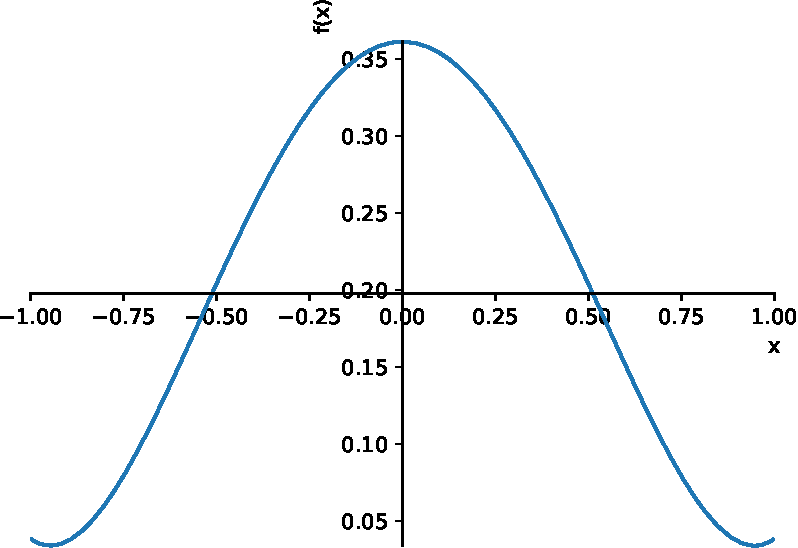
\includegraphics[width = 0.3\textwidth]{chapter_09/exercise_09_48_figure_1.pdf}
  \hspace{1em}
  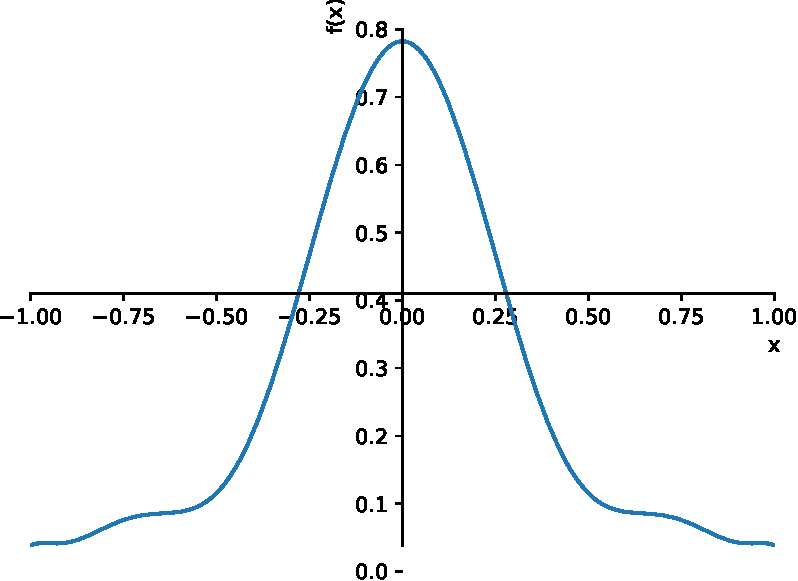
\includegraphics[width = 0.3\textwidth]{chapter_09/exercise_09_48_figure_2.pdf}
  \hspace{1em}
  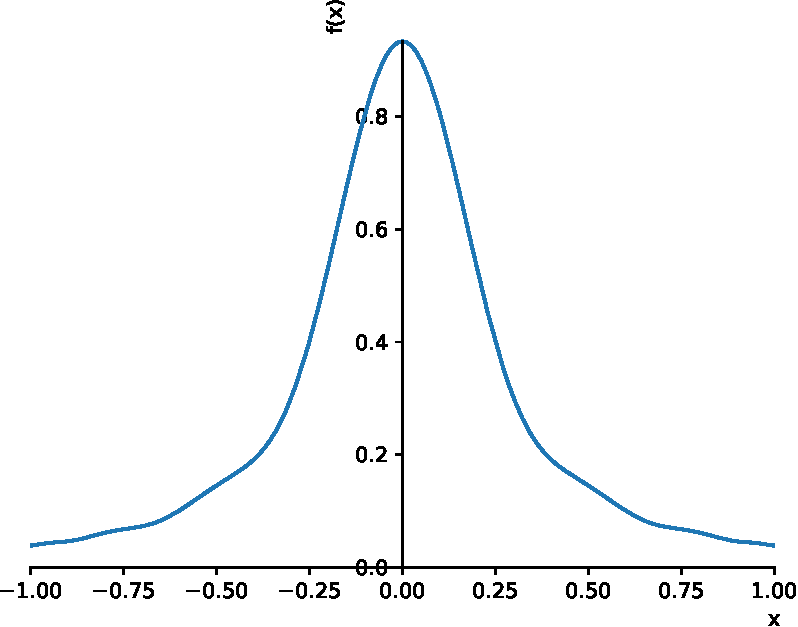
\includegraphics[width = 0.3\textwidth]{chapter_09/exercise_09_48_figure_3.pdf}
\end{center}

Die Oszillationen scheinen für die Chebyshev-Knoten nicht aufzutretten.
Dier ergibt sich auch bei Betrachtung des Fehlers:

\begin{center}
  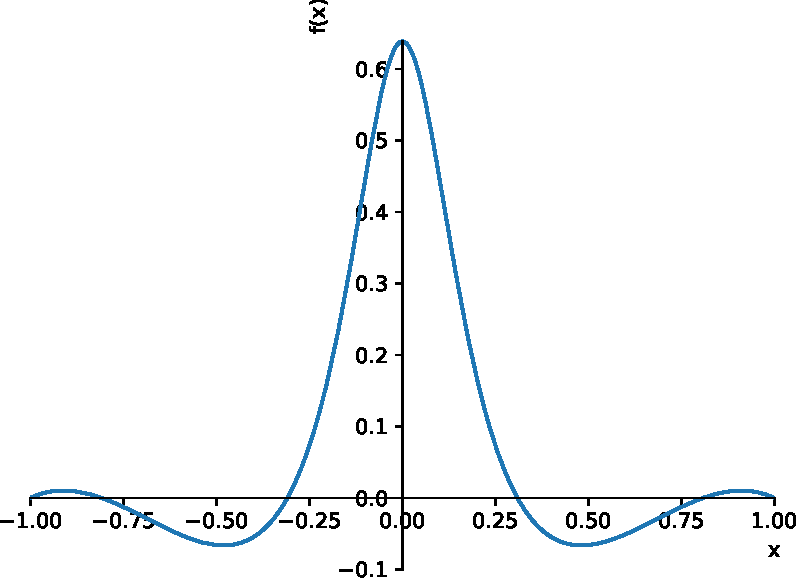
\includegraphics[width = 0.3\textwidth]{chapter_09/exercise_09_48_figure_4.pdf}
  \hspace{1em}
  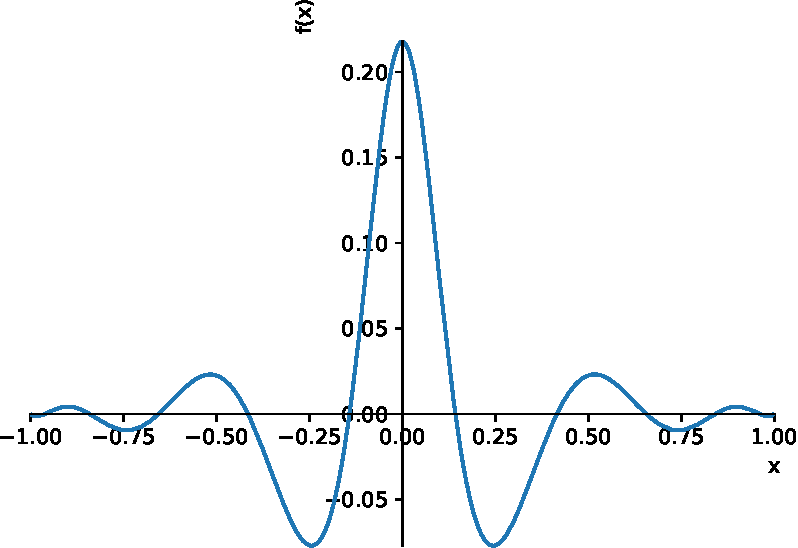
\includegraphics[width = 0.3\textwidth]{chapter_09/exercise_09_48_figure_5.pdf}
  \hspace{1em}
  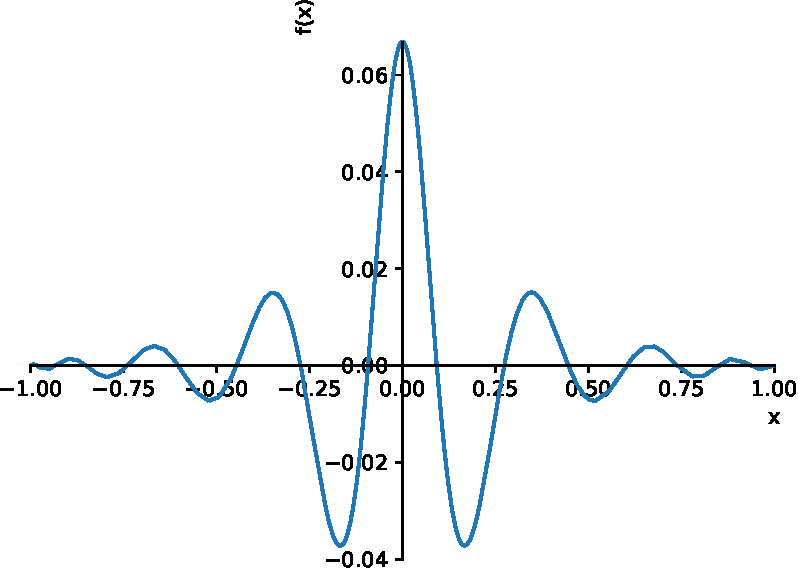
\includegraphics[width = 0.3\textwidth]{chapter_09/exercise_09_48_figure_6.pdf}
\end{center}
